%======================================================================
\chapter{Mobile Device Control}
%======================================================================

%----------------------------------------------------------------------
\section{LQR (P Controller)}
%----------------------------------------------------------------------
\begin{figure}
    \centering
    \subfigure[][]{
    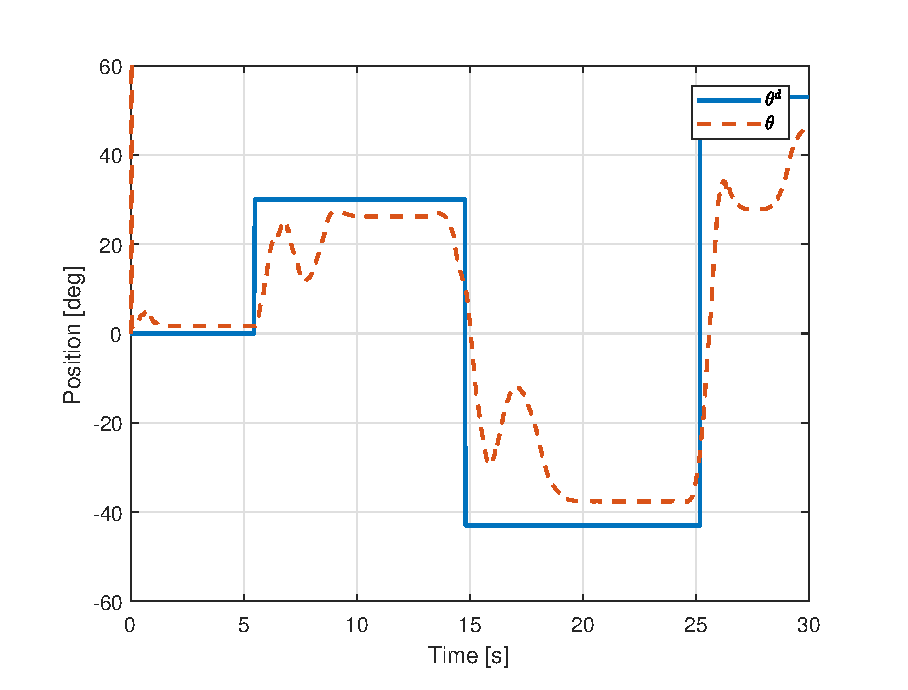
\includegraphics[width=.46\textwidth,keepaspectratio=true]{figs/matlab/LQR/P_Android/LQR_Pitchpos.eps}
    \label{fig:AndroidLQRPitchpos}
    }
    \subfigure[][]{
    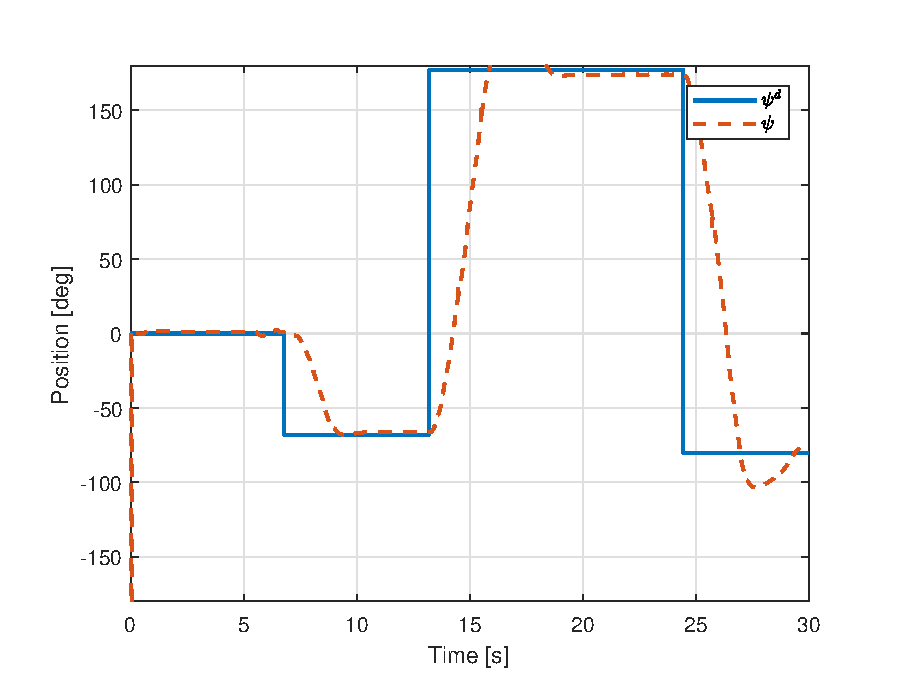
\includegraphics[width=.46\textwidth,keepaspectratio=true]{figs/matlab/LQR/P_Android/LQR_Yawpos.eps}
    \label{fig:AndroidLQRYawpos}
    }
    \subfigure[][]{
    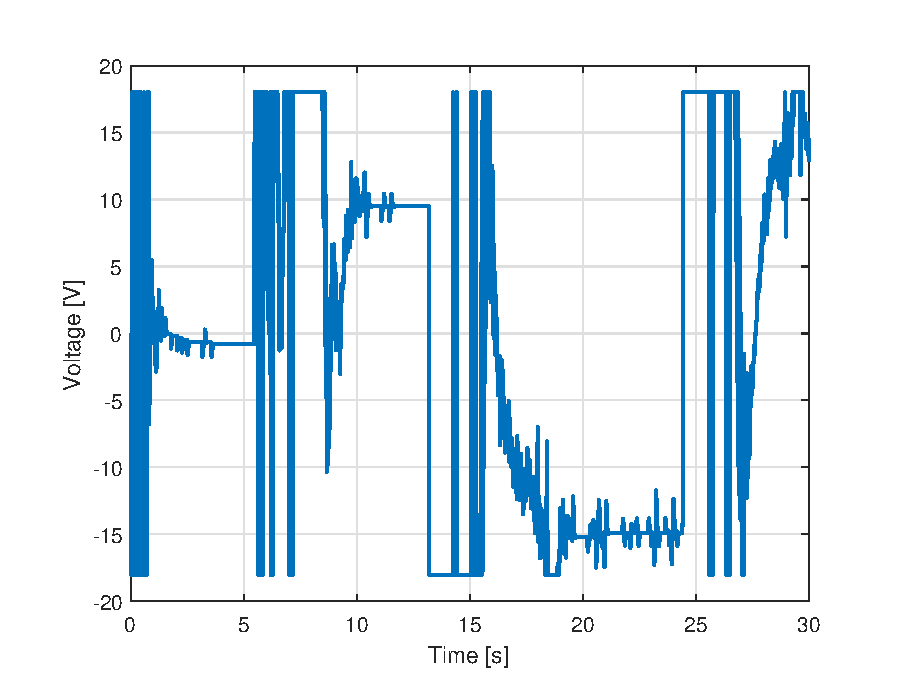
\includegraphics[width=.46\textwidth,keepaspectratio=true]{figs/matlab/LQR/P_Android/LQR_PitchVolt.eps}
    \label{fig:AndroidLQRPitchVolt}
    }
    \subfigure[][]{
    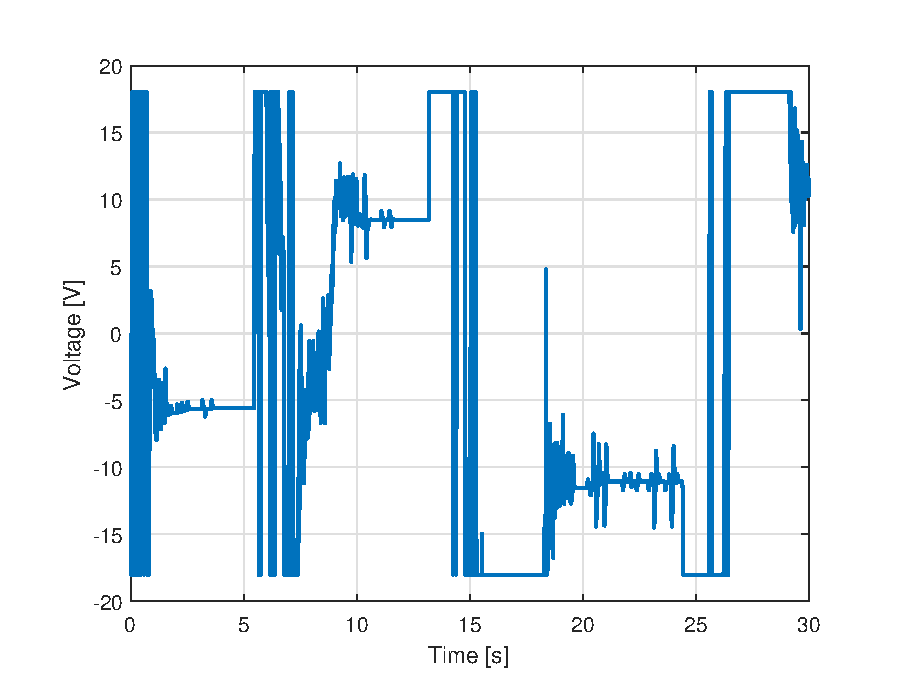
\includegraphics[width=.46\textwidth,keepaspectratio=true]{figs/matlab/LQR/P_Android/LQR_YawVolt.eps}
    \label{fig:AndroidLQRYawVolt}
    }
    \caption{LQR Android Results}
    \label{fig:AndroidLQR}
\end{figure}


%----------------------------------------------------------------------
\section{ADP}
%----------------------------------------------------------------------

\begin{figure}
    \centering
    \subfigure[][]{
    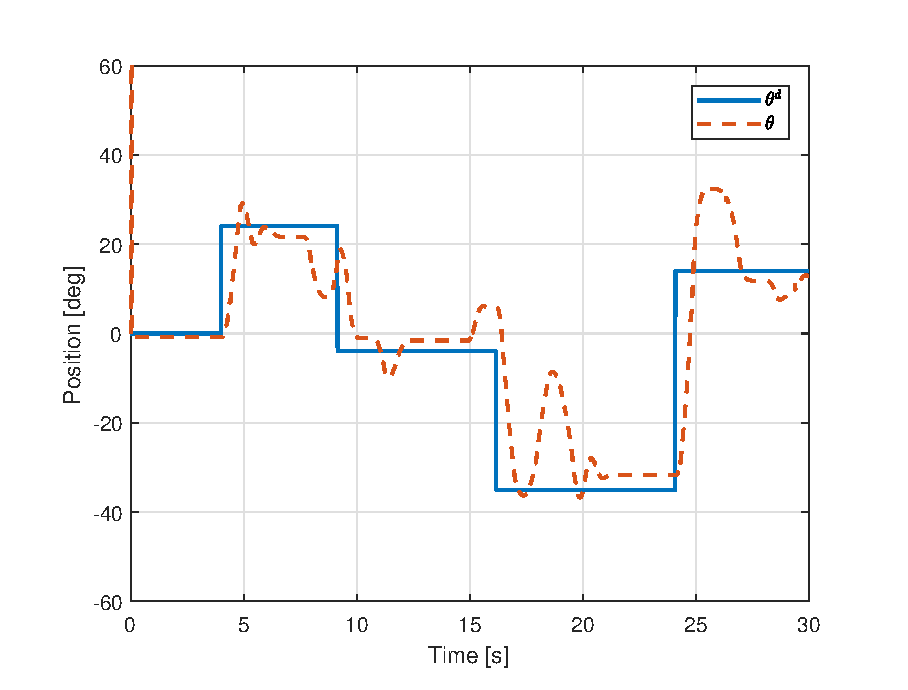
\includegraphics[width=.46\textwidth,keepaspectratio=true]{figs/matlab/ADP/Android/ADP_Pitch_Wireless.eps}
    \label{fig:AndroidADPPitchpos}
    }
    \subfigure[][]{
    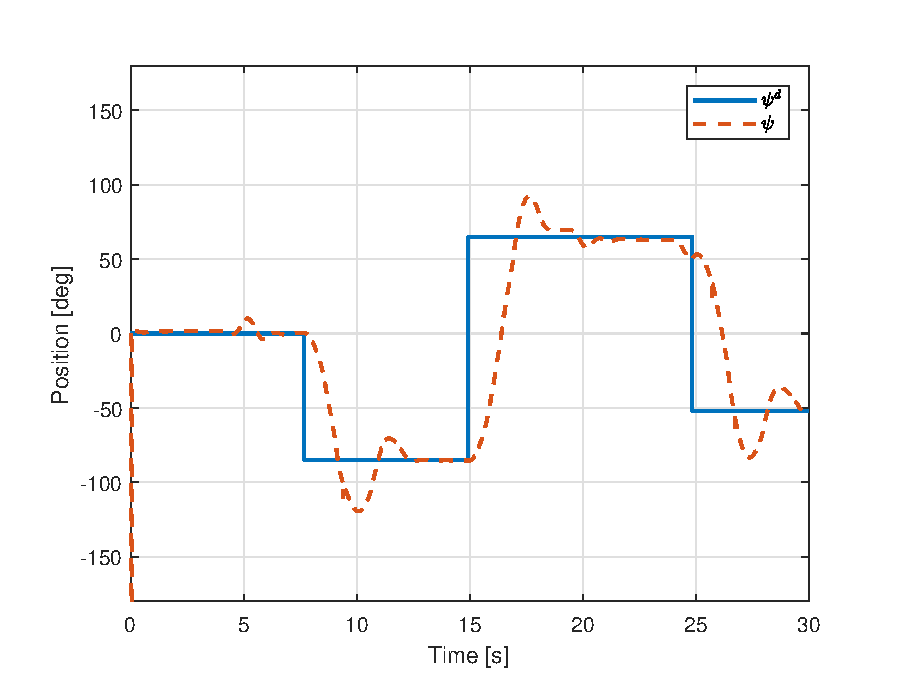
\includegraphics[width=.46\textwidth,keepaspectratio=true]{figs/matlab/ADP/Android/ADP_Yaw_Wireless.eps}
    \label{fig:AndroidADPYawpos}
    }
    \subfigure[][]{
    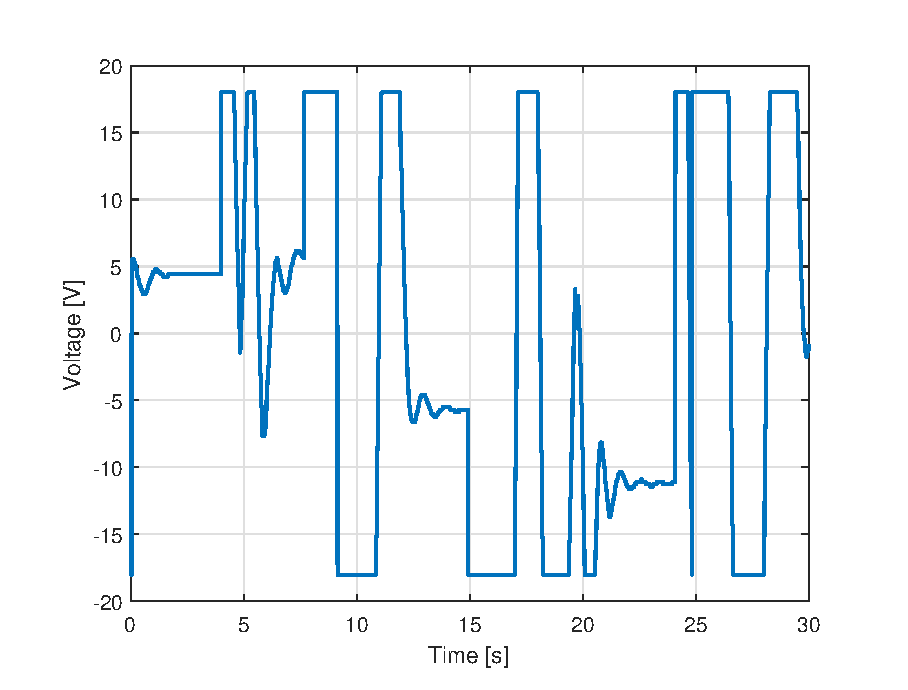
\includegraphics[width=.46\textwidth,keepaspectratio=true]{figs/matlab/ADP/Android/ADP_Pitch_Volt_Wireless.eps}
    \label{fig:AndroidADPPitchVolt}
    }
    \subfigure[][]{
    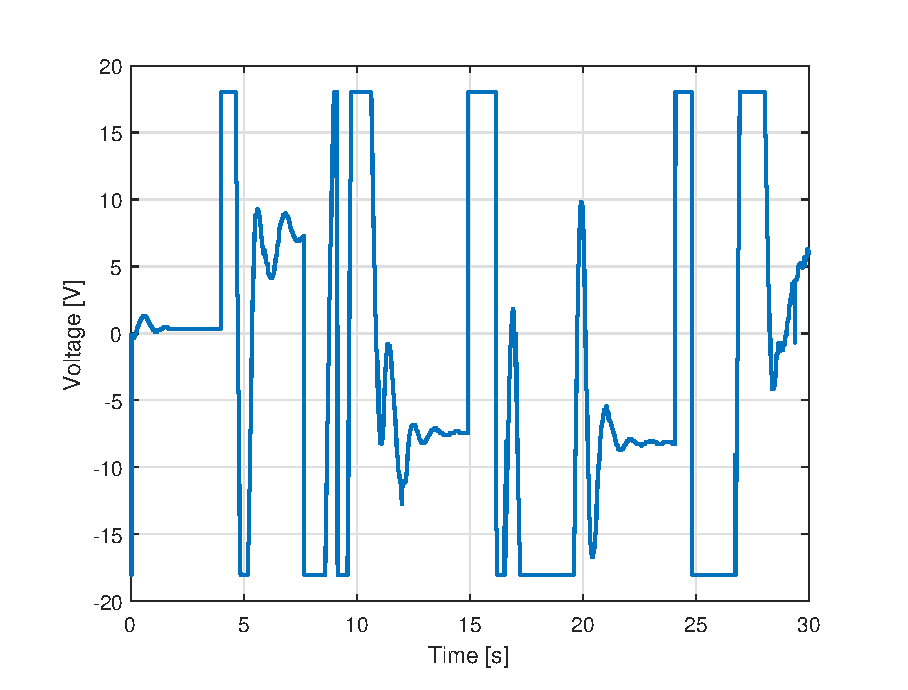
\includegraphics[width=.46\textwidth,keepaspectratio=true]{figs/matlab/ADP/Android/ADP_Yaw_Volt_Wireless.eps}
    \label{fig:AndroidADPYawVolt}
    }
    \caption{ADP Android Results}
    \label{fig:AndroidADP}
\end{figure}

%----------------------------------------------------------------------
\section{Conclusions}
%----------------------------------------------------------------------
Note: constant used pitch XXXX degrees, yaw XXXX degrees\\
Note: square used pitch XXXX degrees with period of XXXX, yaw XXXX degrees with period of XXXX\\
Note: sine used pitch XXXX degrees with period of XXXX, yaw XXXX degrees with period of XXXX\\
\begin{table}[h!]
    \centering
    \begin{tabular}{l|l|l|l|l|l|l}
        \toprule
        \textbf{} & \textbf{LQR(P)} & \textbf{ADP(P)} \\
        \toprule
        RMSE Pitch Step & ? & ?  \\
        RMSE Yaw Step & ? & ? \\
        RMSE Pitch Square & ? & ? \\
        RMSE Yaw Square & ? & ? \\
        RMSE Pitch Sine & ? & ? \\
        RMSE Yaw Sine & ? & ? \\
        \bottomrule
    \end{tabular}
    \caption{Error Comparison for USB Algorithms}
    \label{tab:USB_RMSE}
\end{table}
Based on the results XXXX preformed better for Android.

%----------------------------------------------------------------------



%%% Local Variables:
%%% mode: latex
%%% TeX-master: "../finalReport"
%%% End:
